\documentclass[12pt]{article}
\usepackage{amsmath,mathtools}
\usepackage[usenames,dvipsnames]{xcolor}
%\usepackage[bitstream-charter]{mathdesign}
%\usepackage{mathptmx}

\usepackage{textcomp}
\usepackage{cmbright}
\usepackage[german]{babel}

%\usepackage[activate={true,nocompatibility},final,tracking=true,kerning=true,spacing=true,factor=1100,stretch=10,shrink=10]{microtype}
\usepackage[]{microtype}

\usepackage[utf8]{inputenc}
\usepackage[T1]{fontenc}
%\usepackage{libertine}
%\usepackage{lmodern}

\usepackage{helvet}
\renewcommand{\familydefault}{\sfdefault}
%\usepackage[libertine]{newtxmath}
%\usepackage{graphicx}
\usepackage{siunitx}
%\usepackage{tikz}
\usepackage{fancyhdr}
\usepackage{sectsty}
\usepackage{setspace}
\usepackage{booktabs} % To thicken table lines
\usepackage{chemstyle}
\usepackage[version=4]{mhchem}

%\usepackage[compatibility=4.7,language=german]{chemmacros}

\usepackage[ddmmyyyy]{datetime}
\renewcommand{\dateseparator}{.}
\usepackage{overcite}
\renewcommand\citeform[1]{[#1]}

%\renewcommand*\printatom[1]{{\fontsize{10}{12}\selectfont\ensuremath{\mathsf{#1}}}}
\sectionfont{\fontsize{12}{15}\selectfont}

%\newcommand*\vtick{\textsc{\char13}}

%\expandafter\def\csname libertine@figurestyle\endcsname{LF}

% you can delete this line if you don't use libertine with oldstyle figures:
%\expandafter\def\csname libertine@figurestyle\endcsname{OsF}

%\definesubmol\nobond{[,0.2,,,draw=none]}
%\sectionfont{\fontsize{12}{15}\selectfont}


\newcommand\textbox[1]{%
  \parbox{.333\textwidth}{#1}%
}

\pagestyle{fancy}

\cfoot{\thepage}

\lhead{Nevroz Arslan }
\rhead{\today}
\setlength{\headheight}{15pt}
 \sisetup{
        detect-all %,               %% Benutze gleiche Schriftarten wie im Text
    }
\renewcommand{\thesection}{\arabic{section}.}
\renewcommand{\thesubsection}{\thesection\arabic{subsection}}
\renewcommand{\headrulewidth}{0pt}

\begin{document}


  {\hfil \large \textbf{ Darstellung von 2,2-Diphenylpent-4-ennitril}\hfil}
\par
  \vspace{1cm}
\hfil \textbf{Präparat Nr. 1 von 7}\hfil
\section{Reaktionstyp: \textnormal{ Nukleophile Substitution} }
\begin{scheme}[ht]
\centering
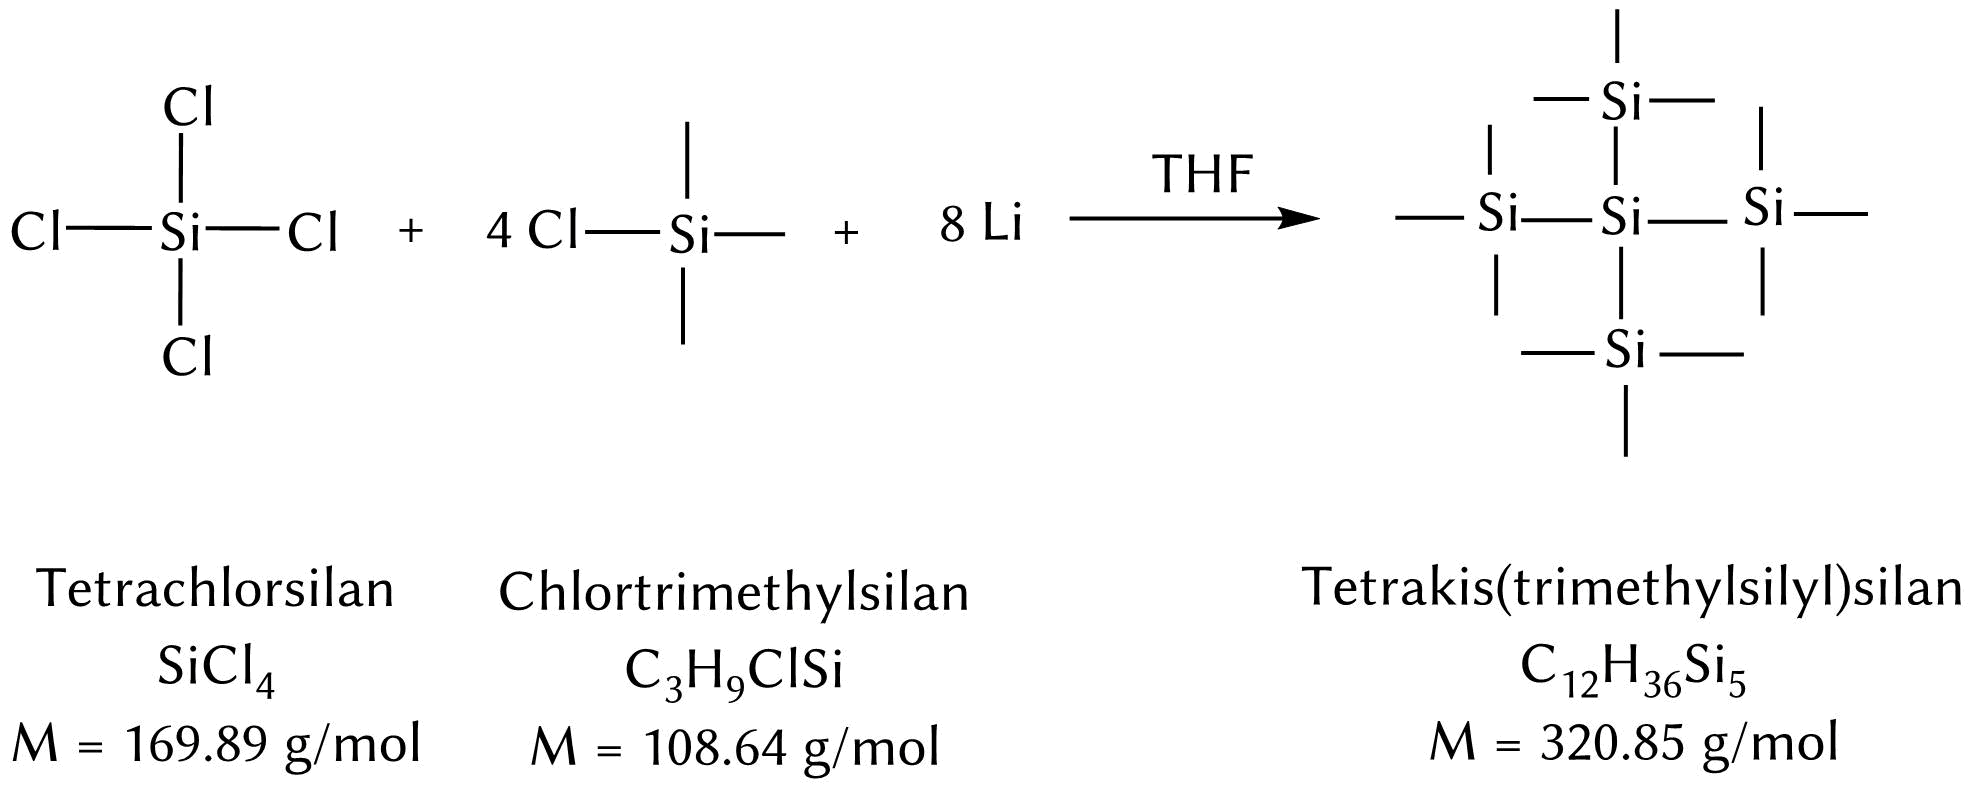
\includegraphics[width=\textwidth]{reaktion}
\end{scheme}

%\chemabove{\lewis{2:,Si}}{\hspace{5mm}\scriptstyle\ominus}
%%%%%%%%%%%%%
% Berechnung des Ansatzes
%%%%%%%%%%%%%
\begin{onehalfspace}

\section{Berechnung des Ansatzes: }
Es sollte 2,2-Diphenylpent-4-ennitril aus Diphenlylacetonitril (19.32 \si{\gram}, 100~\si{\milli\mol}) hergestellt werden. Die Umrechnung des Literaturansatzes ergab folgenden Ansatz:\cite{vor}\\[0.5cm]
\begin{tabular}{lrrrr}
\toprule
\textbf{Bezeichnung }&\textbf{ M [\si{\gram\per\mol}]} & \textbf{n [\si{\milli\mol}]} & \textbf{Menge} & \textbf{Equiv}\\
\midrule
\textit{n}-Butyllithium & 64.05  & 105  & 42 \si{\milli\liter} & 1.05 \\
Diisopropylamin  & 101.19   & 107 &  15 \si{\milli\liter} & 1.07 \\
Allylbromid  & 120.99  & 100   &  8.6 \si{\milli\liter} & 1.00 \\
Diphenylacetonitril & 193.24   & 100  & 19.32 \si{\gram}  & 1.00 \\
THF &   & & 200  \si{\milli\liter}& LM \\
\bottomrule
\end{tabular}\\

%%%%%%%%%%%%%
% Durchführung
%%%%%%%%%%%%%
\normalsize \section{Durchführung \cite{vor}}
Zur Darstellung des 2,2-Diphenyl-pent-4-ennitrils wurden in einem 500 ml-Schlenkkolben eine Lösung von
Diisopropylamin (15 \si{\milli\liter}, 107 \si{\milli\mol}) in Tetrahydrofuran (100~\si{\milli\liter}) vorgelegt
und mit einer Trockeneis-Aceton-Kältemischung auf -78 \si{\celsius} gekühlt. Zu dieser Mischung wurde \textit{n}-Butyllithium (2.5 N, 42 \si{\milli\liter})
zugetropft und die Mischung wurde eine Stunde lang unter Rühren stehen gelassen. Danach
wurde zum Reaktionsgemisch eine Lösung von Diphenylacetonitril (19.32 \si{\gram}, 100 \si{\milli\mol}) in Tetrahydrofuran (50 \si{\milli\liter}) langsam hinzugetropft
und das Gemisch färbte sich gelb. Nach vollständigem Hinzutropfen der Lösung wurde die Apparatur eine weitere halbe Stunde unter Rühren stehen gelassen.
Im Anschluss wurde das Reaktionsgemisch aus dem Kältebad genommen und in ein Eisbad gestellt.
Daraufhin wurde das Gemisch noch 2 Stunden bei 0 \si{\celsius} gerührt.
Danach wurden Allylbromid (8.64 \si{\milli\liter}, 100 \si{\milli\mol}) unter Kühlung im Eisbad in den Reaktionskolben hinzugegeben
und der Kolbeninhalt wurde über Nacht bei Raumtemperatur gerührt.
Dann wurde die Reaktionslösung mit Ammoniumchloridlösung (10 \%ig, 150 \si{\milli\liter}) hydrolysiert und die wässrige Phase mit Diethylether (2 x 100 \si{\milli\liter}) extrahiert.
Nach dem Trocknen über Magnesiumsulfat wurde das Lösungsmittel im Rotationsverdampfer entfernt und
 das Rohprodukt an der Hochvakuumpumpe getrocknet. Das Produkt (20.75 g, 88.9 mmol, 89 \%) wurde als gelbe Flüssigkeit erhalten.
%%%%%%%%%%%%
% Ausbeute
%%%%%%%%%%%%%
\section{Ausbeute}
\begin{tabular}{ ll}
  23.33 g (100.0 mmol)   & = 100 \%\\
  20.75 g (88.9 mmol)    & = 89 \% (Lit.\cite{vor} : 99 \%) \\
 \end{tabular}
 \pagebreak
%%%%%%%%%%%%%
%Physikalische Daten des Produktes
%%%%%%%%%%%%%
%\section{Physikalische Daten des Produktes}
%\textit{2,2-Dimethyl-pent-4-enenitril}
\section{Spektrenauswertung}

\begin{scheme}[!ht]
   \centering
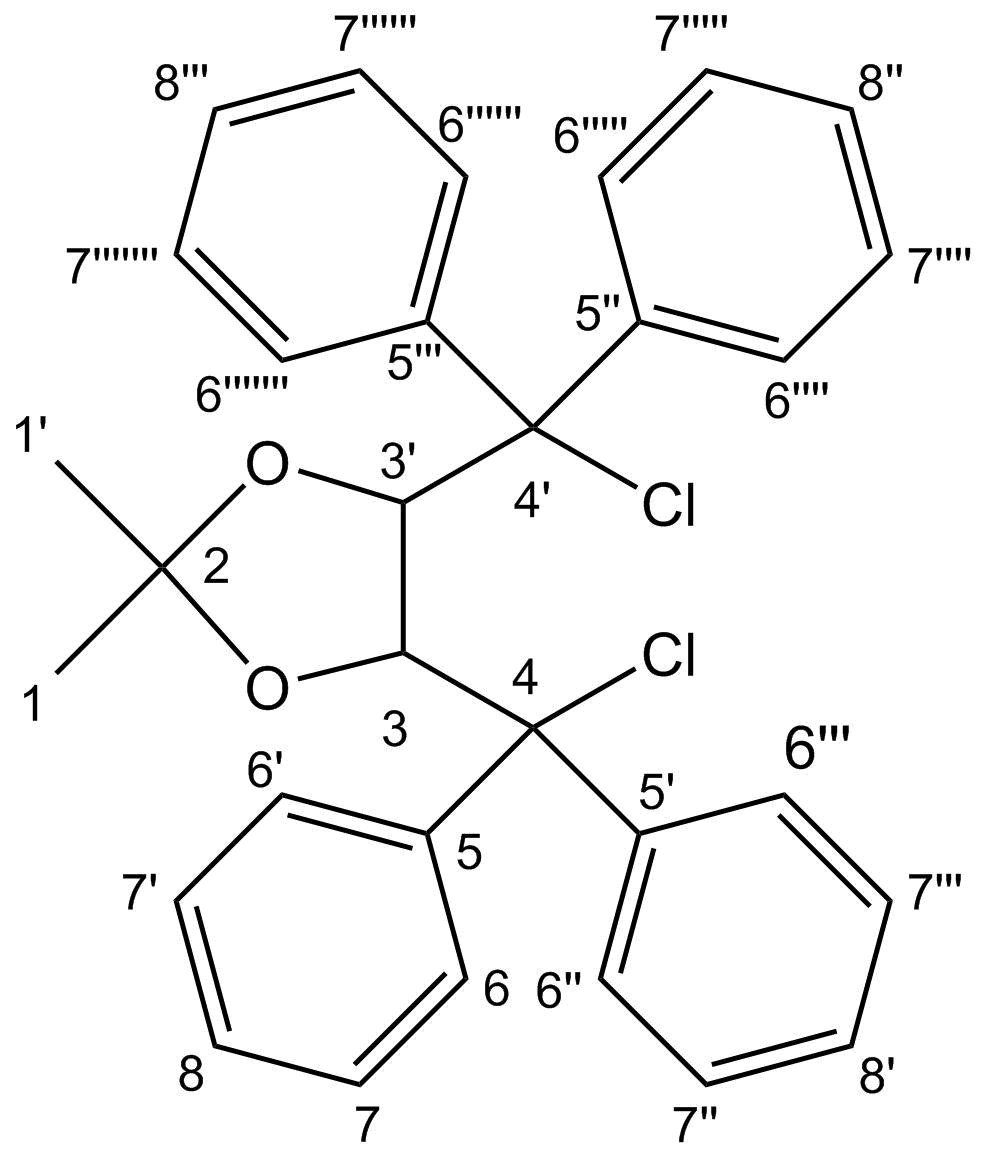
\includegraphics{auswert}
\end{scheme}
\noindent
\textbf{\ce{^1_{}H-NMR}} (300 MHz, \ce{CDCl_3}): \sffamily \ce{$\delta$} =
3.06 (d, \ce{^3_{}\textit{J}} = 15.9 \si{\hertz}, 2 H, 3-H),
5.05 - 5.19 (m, 2 H, 3-H),
5.64 (ddt, \ce{^3_{}\textit{J}} = 7.0 \si{\hertz}, \ce{^3_{}\textit{J}_{cis}} = 10.1 \si{\hertz}, \ce{^3_{}\textit{J}_{trans}} = 17.1 \si{\hertz}, 1 H, 4-H),
7.12-7.50 (m, 10 H, 6-H, 7-H, 8-H, 9-H) ppm.

\section{Mechanismus\cite{bio}}
Im ersten Teil der Reaktion erfolgt eine metallierung des Amins \textbf{2}. Die starke Base \textit{n}-Butyllithium (\textbf{1}) vermag das
H-Atom des Amins als Proton abzulösen.
Treibende Kraft dieser Säure-Base-Reaktion ist das Bestreben des Lithiums, die
acidere Position einzunehmen. Es bildet sich eine starke Base \textbf{3} mit den sperrigen Isopropyl-Substituenten.\\
Im zweiten Teil der Reaktion erfolgt die Deprotonierung einer CH-Aciden Verbindung.
Das Diisopropylamidanion \textbf{3} deprotoniert das Diphenylacetonitril (\textbf{4}) und
es entsteht das Carbanion \textbf{5}. Das Carbanion \textbf{5} wird durch die Mesomerie der Phenlygruppen und Nitrilgruppe stark stabilisiert.\\
Im dritten Teil der Reaktion erfolgt eine nukleophile Substitution. Das entstandene nukleophile Diphenylacetonitrilanion (\textbf{5}) greift
 Allylbromid (\textbf{6}) am elektrophilen Kohlenstoffatom an. Unter Abspaltung von \ce{LiBr} entsteht das gewünschte Produkt 2,2-Diphenylpent-4-ennitril (\textbf{7}).
 \newpage
 \begin{scheme}[!ht]
   \centering
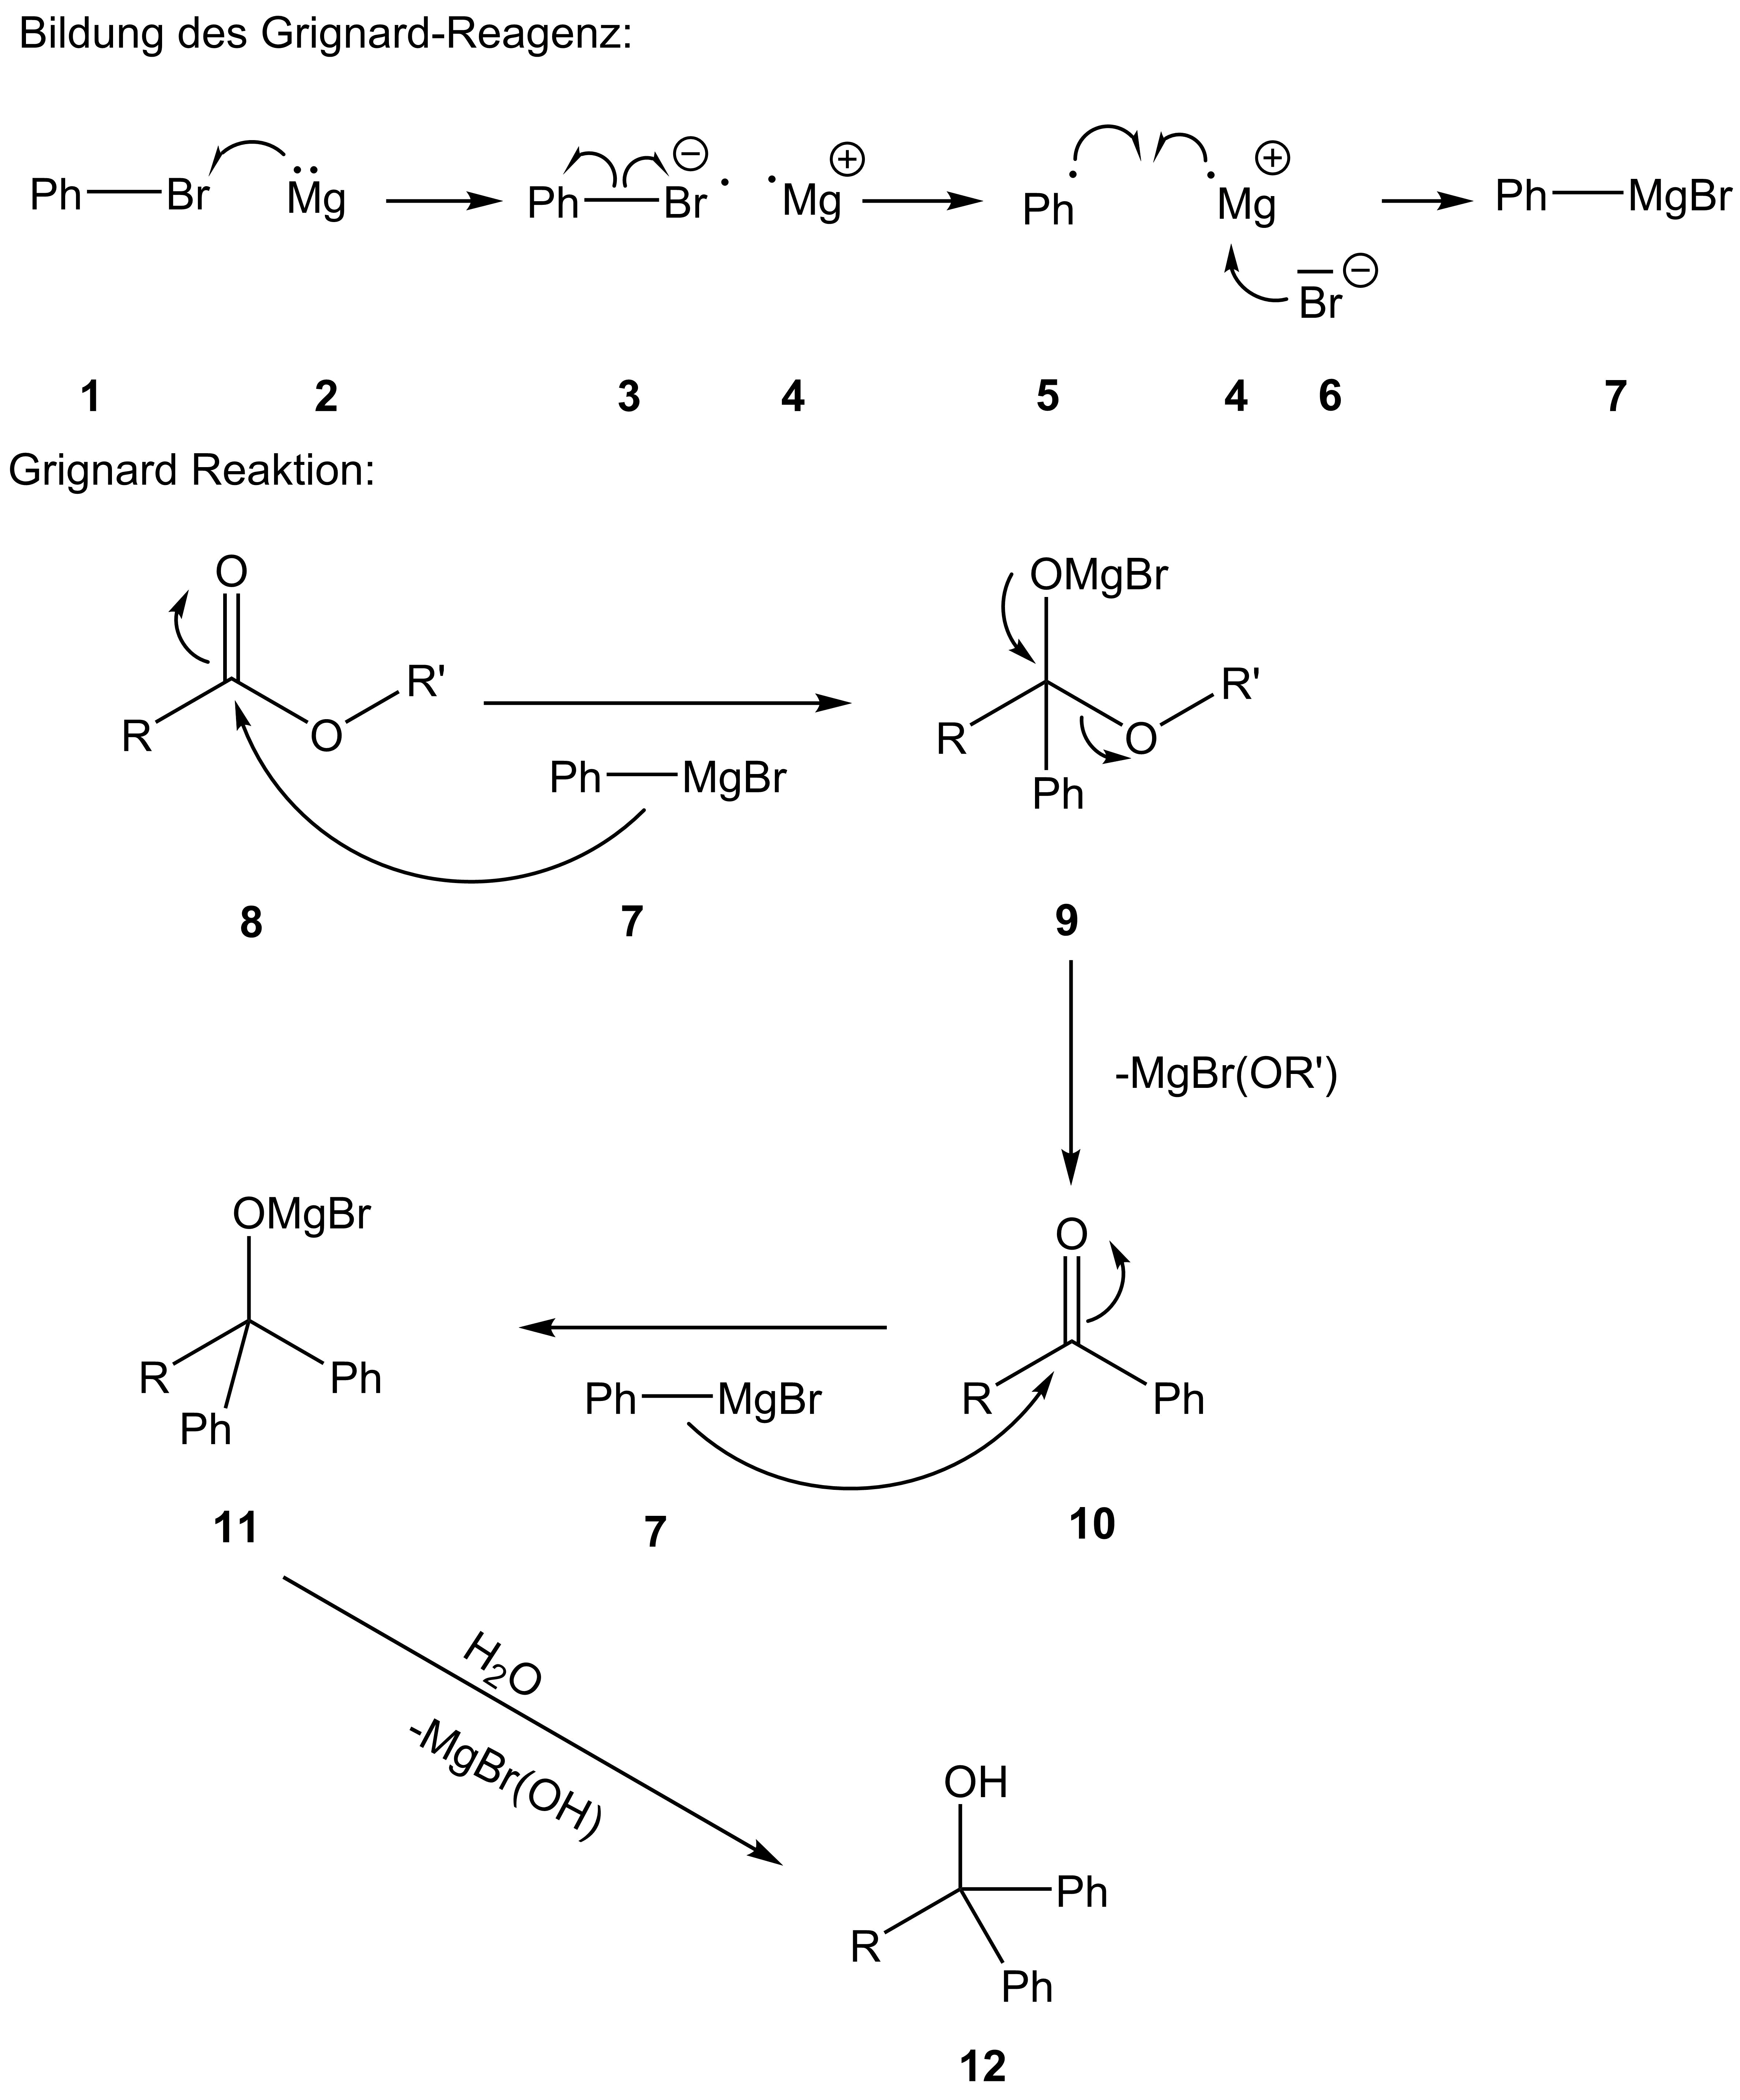
\includegraphics[width=\textwidth]{mechan}
\end{scheme}
\section{Abfallentsorgung}
Die nach dem Waschen mit Ammoniumchloridlösung und Wasser verbleibenden wässrigen Phasen wurden nach einer pH-Wertbestimmung im Behälter für saure wässrige Abfälle entsorgt.
Das im Rotationsverdampfer abgetrennte Lösungsmittel wurde im Behälter für halogenfreie Kohlenwasserstoffe entsorgt.
\section{Literatur}
\renewcommand{\section}[2]{}%

\def\bibindent{0em}
\begin{thebibliography}{99\kern\bibindent}
\makeatletter
\let\old@biblabel\@biblabel
\def\@biblabel#1{\old@biblabel{#1}\kern\bibindent}
\let\old@bibitem\bibitem
\def\bibitem#1{\old@bibitem{#1}\leavevmode\kern-\bibindent}
\makeatother
\bibitem{vor}
P. Martinez, K. C. Hultzsch, F. Hampel, \textit{Chem. Commun.} \textbf{2006}, 2221 - 2223.
%H. Becker, W. Berger, G. Domschke, E. Fanghänel, J. Faust, M. Fischer, F. Gentz, K. Gewald, R. Gluch, R. Mayer, K. Müller, D. Pavel, H. Schmidt, K. Schollberg, K. Schwetlick, E. Seiler, G. Zeppenfeld, R. Beckert, G. Domschke, W. Habicher, P. Metz, \textit{bio}, 21. Aufl., Wiley-VCH, Weinheim \textbf{2009}, S. 521-522.
\bibitem{bio}
J. Buddrus, \textit{Grundlagen der Organische Chemie}, 4. Aufl., De Gruyter, Berlin \textbf{2011}, S. 258, 701.
\end{thebibliography}
\end{onehalfspace}
\end{document}


